\documentclass[a4paper,11pt]{article}
\usepackage{polski}
\usepackage[utf8]{inputenc}

% \usepackage{a4wide}

\usepackage{amsmath}
\usepackage{amsfonts}
% \usepackage{amssymb}
% \usepackage{amsthm}
\usepackage{listings}
\usepackage{graphicx}

\title{
  \textbf{Pracownia 30}\\
  {\Large Podstawy elektroniki, elektrotechniki i miernictwa}
}
\author{Rafał Łasocha}
\setcounter{equation}{0}

\begin{document}

\maketitle

\section{Zagadnienia teoretyczne}

\subsection{Bramki elementarne}

\subsubsection{Bramka OR}
Bramka OR jest bramką z dwoma wejściami i jednym wyjściem, wg następującej tabeli prawdy:

\begin{center}
	\begin{tabular}{|l|l|l|}\hline
	$We_1$ & $We_2$ & $Wy$ \\ \hline
	0 & 0 & 0 \\
	0 & 1 & 1 \\
	1 & 0 & 1 \\
	1 & 1 & 1 \\ \hline
	\end{tabular}
\end{center}

\subsubsection{Bramka AND}
Bramka AND jest bramką z dwoma wejściami i jednym wyjściem, wg następującej tabeli prawdy:

\begin{center}
	\begin{tabular}{|l|l|l|}\hline
	$We_1$ & $We_2$ & $Wy$ \\ \hline
	0 & 0 & 0 \\
	0 & 1 & 0 \\
	1 & 0 & 0 \\
	1 & 1 & 1 \\ \hline
	\end{tabular}
\end{center}

\subsubsection{Bramka NOT}
Bramka NOT jest bramką z jednym wejściem i jednym wyjściem, wg następującej tabeli prawdy:

\begin{center}
	\begin{tabular}{|l|l|}\hline
	$We$ & $Wy$ \\ \hline
	0 & 1 \\
	1 & 0 \\ \hline
	\end{tabular}
\end{center}

\subsection{Przerzutnik R-S}
Jest to najpopularniejsza wersja przerzutnika. Jego działanie opiera się na dwóch bitach, Set i Reset. ustawienie Set na 1, ustawia wartość 1 na przerzutniku, a ustawienie Reset na 1, ustawia wartość 0 na przerzutniku. Nie ustawienie żadnego z tych bitów oznacza utrzymanie aktualnego stanu. Ustawienie zarówno Set jak i Reset jednocześnie jest niedozwolone.

\begin{center}
	\begin{tabular}{|l|l|l|l|}\hline
	$S$ & $R$ & $Q_n$ & $!Q_n$ \\ \hline
	0 & 0 & $Q_{n-1}$ & $!Q_{n-1}$ \\
	1 & 0 & 1 & 0 \\
	0 & 1 & 0 & 1 \\
	1 & 1 & - & - \\ \hline
	\end{tabular}
\end{center}


\subsection{Synchroniczny przerzutnik R-S}
Przerzutnik synchroniczny ma dodatkowe wejście zegara. Synchroniczny przerzutnik R-S nie zmienia swojej wartości od razu, tylko synchronicznie z danym zegarem.

\subsection{Przerzutnik JK}
Rodzaj przerzutnika synchronicznego. Ma podobne tabele wzbudzeń jak przerzutnik R-S, jednak posiada dwa dodatkowe wejścia działające asynchronicznie.

\subsection{Przerzutnik D}
Jest to przerzutnik synchroniczny, działający wg następującej tabeli prawdy.

\begin{center}
	\begin{tabular}{|l|l|l|}\hline
	$D$ & $Q(t)$ & $Q(t+1)$ \\ \hline
	0 & 0 & 0 \\
	0 & 1 & 0 \\
	1 & 0 & 1 \\
	1 & 1 & 1 \\ \hline
	\end{tabular}
\end{center}

\subsection{Rejestr przesuwający}
Rejestr zbudowany z przerzutników w taki sposób, że w takt impulsów wejścia zegara informacja bitowa przesuwa się po kolejnych przerzutnikach.

\section{Przebieg ćwiczenia}

\subsection{Przerzutniki R-S}

Pierwszą częścią ćwiczenia było zbudowanie przerzutników R-S jak przedstawiono na rysunku 1. Pierwszy z układów miał tabelę prawdy taką samą jak przedstawiono w przerzutniku R-S w zagadnieniach teoretycznych. Drugi z układów miał wyjścia przeciwne. Oznacza to, że był to przerzutnik z wejściami zanegowanymi, jednak taki przerzutnik ma dokładnie taką samą funkcjonalność jak zwykły przerzutnik R-S.

\begin{figure}[ht]
 \begin{center}
  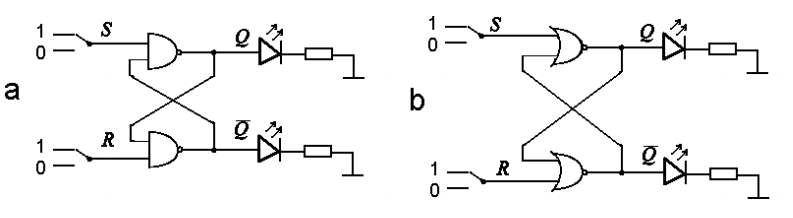
\includegraphics[width=12cm]{screenshot135}
 \end{center}
 \caption{Przerzutniki R-S}
\end{figure}

\subsection{Przerzutniki synchroniczne}

Następnie zbudowaliśmy układy z rysunku 2. Po tabelach wzbudzeń można wywnioskować że był to odpowiednio przerzutnik synchroniczny R-S i przerzutnik D.

\begin{figure}[ht]
 \begin{center}
  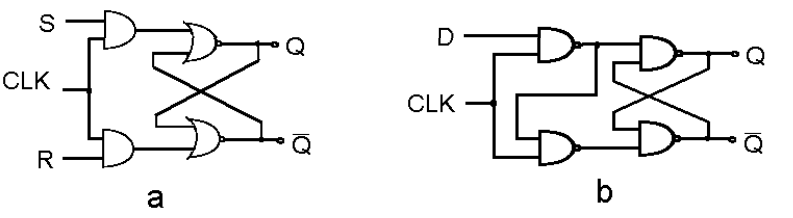
\includegraphics[width=12cm]{screenshot134}
 \end{center}
 \caption{Przerzutniki synchroniczne}
\end{figure}

\subsection{Rejestr przesuwający}
Przedostatnim zadaniem było zbudowanie prostego rejestru przesuwającego z wejściem szeregowym oraz wyjściami równoległymi i szeregowym zgodnie z rysunkiem 3.

\begin{figure}[ht]
 \begin{center}
  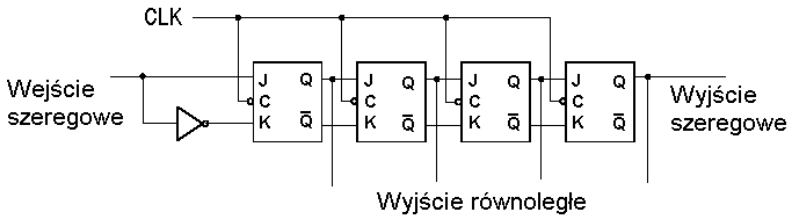
\includegraphics[width=12cm]{screenshot133}
 \end{center}
 \caption{Rejestr przesuwający}
\end{figure}

\subsection{Licznik binarny}
Dodatkowym zadaniem było zrobienie z 4 przerzutników JK licznika binarnego. Układ miał działać w ten sposób, że licznik binarny (złożony z czterech diód) miał zwiększać wartość o 1 za każdym razem gdy użytkownik wysłał impuls.



\section{Wnioski}



\end{document}